
\begin{figure}[H]
\centering
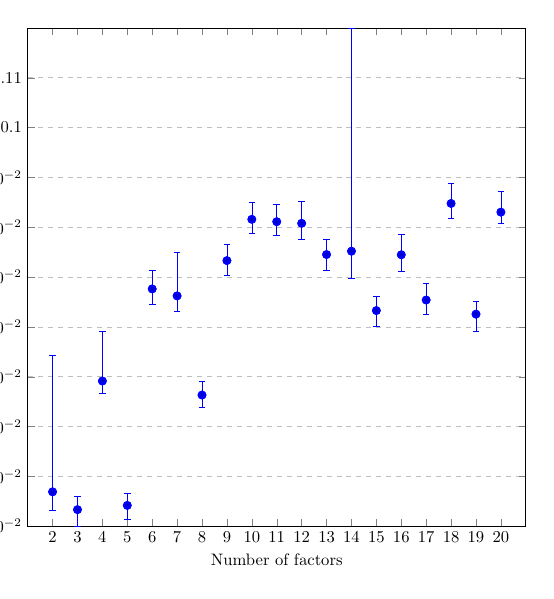
\begin{tikzpicture}[scale=0.6, trim axis left, trim axis right]
\begin{axis}[
    width=1\textwidth,
    height=1\textwidth,
    xlabel={Number of factors},
    ylabel={Time taken (s)},
    xmin=1.0, xmax=21.0,
    ymin=0.058421, ymax=0.111037,
    xticklabels={2, 3, 4, 5, 6, 7, 8, 9, 10, 11, 12, 13, 14, 15, 16, 17, 18, 19, 20},
    xtick={2, 3, 4, 5, 6, 7, 8, 9, 10, 11, 12, 13, 14, 15, 16, 17, 18, 19, 20},
    ytick={0.058421, 0.0636826, 0.0689442, 0.0742058, 0.0794674, 0.084729, 0.0899906, 0.0952522, 0.1005138, 0.1057754},
    ymajorgrids=true,
    grid style=dashed,
]

\addplot+[
    blue,
    very thick,
    forget plot,
    only marks
    ]
    plot[
    very thick,
    error bars/.cd,
    y dir=plus,
    y explicit
    ]
    table[x=x,y=y,y error expr=\thisrow{y-max}] {
    x    y    y-max
    11	0.0905798666667	0.00180913333333
10	0.0908301333333	0.00176886666667
13	0.0871118	0.0016222
12	0.0904066333333	0.00227636666667
15	0.0811915333333	0.00149346666667
14	0.0874642333333	0.0235727666667
17	0.0823064333333	0.00180656666667
16	0.0870842	0.0022068
19	0.0808105333333	0.00139446666667
18	0.0925048	0.0021542
20	0.0915868	0.0021572
3	0.0601651333333	0.00138586666667
2	0.0620452	0.0144208
5	0.0606133	0.0012837
4	0.0737501	0.0052569
7	0.0827417333333	0.00455026666667
6	0.0834780666667	0.00200193333333
9	0.0864688666667	0.00173713333333
8	0.0722704	0.0014106

    };

\addplot+[
    blue,
    very thick,
    forget plot,
    only marks
    ]
    plot[
    very thick,
    error bars/.cd,
    y dir=plus,
    y explicit
    ]
    table[x=x,y=y,y error expr=\thisrow{y-min}] {
    x    y    y-min
    11	0.0905798666667	-0.00145286666667
10	0.0908301333333	-0.00146313333333
13	0.0871118	-0.0016858
12	0.0904066333333	-0.00171563333333
15	0.0811915333333	-0.00166953333333
14	0.0874642333333	-0.00284223333333
17	0.0823064333333	-0.00153443333333
16	0.0870842	-0.0017692
19	0.0808105333333	-0.00184853333333
18	0.0925048	-0.0015858
20	0.0915868	-0.0012168
3	0.0601651333333	-0.00174413333333
2	0.0620452	-0.0019012
5	0.0606133	-0.0014973
4	0.0737501	-0.0012571
7	0.0827417333333	-0.00161973333333
6	0.0834780666667	-0.00166306666667
9	0.0864688666667	-0.00156886666667
8	0.0722704	-0.0012644

    };

\end{axis}
\end{tikzpicture}
\vspace{-0.3cm}
\caption{Large primes, modified algorithm}\label{fig:TrialDivisionlargeprimes(modified:True)factors}
\end{figure}
